\section{Modelo}
\label{sec:modelo}

Un modelo de aprendizaje automático de clasificación es un sistema computacional diseñado para aprender patrones en los datos y realizar predicciones en base a esos patrones sin tentar que ser programado explícitamente para cada tarea. 

Uno de los principales problemas al aplicar estos métodos a señales EEG es la gran disparidad existente entre los distintos conjuntos de datos disponibles, especialmente en datasets públicos. Estas diferencias abarcan aspectos como la disposición y el número de electrodos, la duración de los periodos de imaginación motora, las acciones de imaginación motora diferenciadas, la frecuencia de muestreo y, de manera especialmente relevante, los formatos de almacenamiento de los datos y la nomenclatura utilizada tanto para los eventos como para las posiciones de los electrodos.

Esta heterogeneidad dificulta significativamente la integración de múltiples datasets, limitando la posibilidad de reunir grandes volúmenes de datos para el entrenamiento. Como consecuencia, suele ser necesaria una adaptación manual o semiautomática de cada conjunto de datos, con el fin de unificarlos y permitir que un mismo modelo pueda aprender de todos ellos de manera coherente.

Por esta razon se buscó un modelo que proporcionase pesos preentrenados y que solo necesitase un fineTuning con la menor cantidad de datos posibles para adaptarse a un sujeto en concreto.

Históricamente, los primeros modelos de aprendizaje automático aplicados a interfaces cerebro-computador (BCI) se basaban en arquitecturas importadas de otros dominios, especialmente de la visión por computador, sin una adaptación específica a las características propias de las señales EEG. Posteriormente, surgieron modelos diseñados específicamente para este tipo de señales, como EEGNet, cuya arquitectura incorpora mecanismos orientados a capturar tanto patrones temporales como espaciales característicos del EEG.

No obstante, estos modelos suelen entrenarse en escenarios con una cantidad limitada de datos, ya sea a nivel intra-sujeto o utilizando datasets relativamente pequeños, lo que limita su capacidad de generalización. Con el objetivo de abordar esta limitación, han surgido los denominados modelos fundacionales, que buscan aprender representaciones generales a partir de grandes colecciones de datos. Para ello, estos modelos suelen combinar múltiples datasets, en ocasiones pertenecientes a distintos paradigmas BCI, y posteriormente adaptarse a tareas específicas mediante técnicas de fine-tuning.

Sin embargo, la mezcla de datos procedentes de diferentes paradigmas puede resultar problemática debido a las diferencias neurofisiológicas existentes entre ellos, lo que puede afectar negativamente a la calidad de las representaciones aprendidas. En este contexto, MiRepNet se plantea como un modelo fundacional especializado en imaginación motora, entrenado exclusivamente con datasets de este paradigma. De este modo, busca aprender patrones generales específicos de la imaginación motora que permitan, mediante FineTuning con una cantidad reducida de datos, adaptarse eficazmente a nuevos sujetos.

MiRepNet es un modelo de aprendizaje profundo basado en la arquitectura transformer y especializado en EEG que proporciona pesos preentrenados sobre 50.355 trials y clasifica 4 clases de imaginación motora siendo estas: mano izquierda, mano derecha, pies y lengua.

\subsection{Arquitectura basada en transformer}
\label{subsec:arquitecturaModelo}

MiRepNet se compone de tres bloques principales que actúan de forma secuencial: un tokenizador que convierte la señal EEG en una secuencia de representaciones vectoriales, un encoder transformer que modela las relaciones entre dichas representaciones, y una cabeza de clasificación que produce la predicción final. A continuación se describe cada uno de estos componentes.

\subsubsection{Estructura tokenizador}
\label{subsubsec:arquitecturaTockenizador}

La arquitectura de MiRepNet está basada en la arquitectura transformer. Primero los datos son transformados en tockens que posteriormente son procesados por un transformer. 

El proceso del tokenizer comienza con la señal de entrada representada como una matriz de dimensiones $C \times T$, donde $C$ corresponde al número de canales (electrodos) y $T$ al número de muestras temporales.

En primer lugar, se aplica una convolución temporal, compuesta por 64 filtros entrenables, que opera a lo largo del eje temporal de cada canal de forma independiente. Esta operación permite al modelo aprender patrones temporales característicos de la señal EEG, como ritmos específicos (por ejemplo, bandas de frecuencia) o la atenuación de ruido.

A continuación, sobre la representación generada se aplica una convolución espacial compuesta por 128 filtros entrenables, cuyo objetivo es capturar las relaciones entre los distintos canales. En este caso, los filtros se aplican a lo largo del eje de canales, combinando la información procedente de distintos electrodos. Como resultado, se obtienen nuevas representaciones que integran la información espacial del EEG, permitiendo al modelo identificar patrones distribuidos en diferentes regiones del cuero cabelludo además de eliminar la dimensión de los canales para las siguientes transformaciones.

Posteriormente, se aplica una operación de normalización junto con la función de activación ELU, con el objetivo de estabilizar el proceso de entrenamiento e introducir no linealidad en el modelo, permitiendo así la representación de patrones más complejos.

A continuación, se emplea una operación de average pooling para reducir la dimensión temporal de las representaciones, lo que permite disminuir la cantidad de datos a procesar y mejorar la eficiencia del modelo.

Tras esta etapa, se obtienen un conjunto de vectores que contienen información espaciotemporal resumida de la señal EEG. Sobre estos vectores se aplica una capa de proyección, implementada mediante una convolución, cuyo objetivo es transformar las representaciones al espacio de dimensión fija definido por el embedding dimension.

Finalmente, los tokens se construyen tomando, para cada instante temporal, los valores de todos los filtros, de modo que cada token la información espacio-temporal completa obtenida mediante las convoluciones para un instante. 

\subsubsection{Estructura pretraining}
\label{subsubsec:arquitecturaEntrenamiento}

\begin{figure}[h]
	\centering
	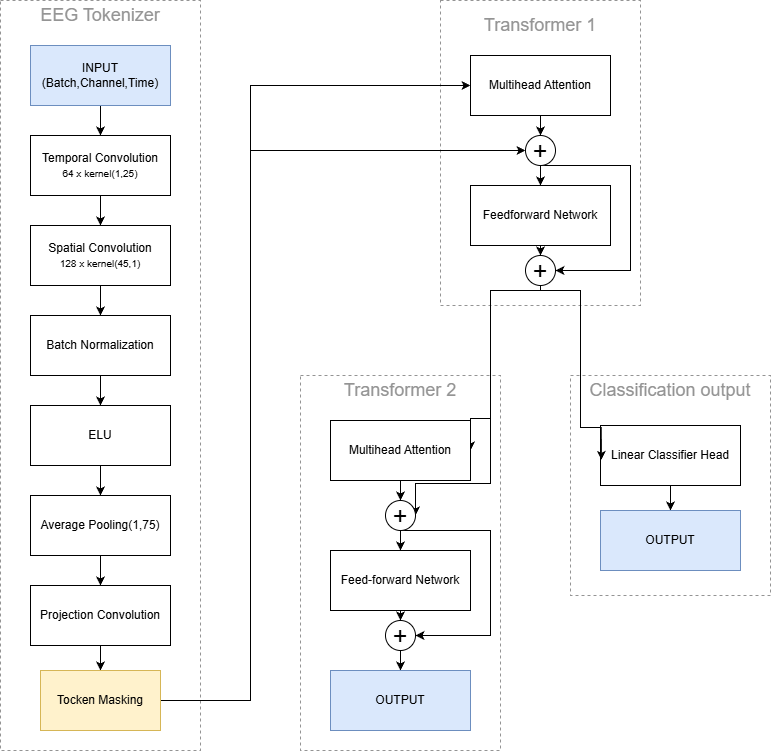
\includegraphics[width=\textwidth]{Imagenes/Bitmap/Esquema-Training-Modelo}
	\caption{Esquema de la arquitectura de MiRepNet para entrenamiento.}
	\label{fig:esquemaTrainingModelo}
\end{figure}

Durante la fase de pretraining, el modelo combina aprendizaje supervisado y no supervisado con el objetivo de mejorar la calidad de las representaciones aprendidas. Para ello, en primer lugar se oculta una parte de los tokens de entrada, generando así una tarea de reconstrucción.

Los datos son procesados inicialmente por un bloque Transformer compuesto por un módulo de multi-head attention, encargado de modelar las relaciones entre los tokens, y una red feedforward. Ambos subbloques están precedidos por una operación de normalización y emplean conexiones residuales, de modo que la salida de cada subbloque se suma a su entrada. Este primer Transformer tiene como objetivo aprender representaciones generales de las señales EEG en tareas de imaginación motora.

La salida de este bloque se bifurca en dos ramas. Por un lado, se aplica una transformación lineal para realizar la predicción de la tarea supervisada (clasificación). Por otro lado, las representaciones se introducen en un segundo bloque Transformer, con la misma estructura que el anterior, cuyo objetivo es reconstruir los tokens previamente ocultos. Esta segunda rama constituye la parte no supervisada del entrenamiento.

Finalmente, el modelo se entrena mediante la optimización conjunta de ambas tareas, combinando las pérdidas asociadas a la clasificación y a la reconstrucción.

\subsubsection{Estructura Downstream}
\label{subsubsec:arquitecturaDownstream}

\begin{figure}[h]
	\centering
	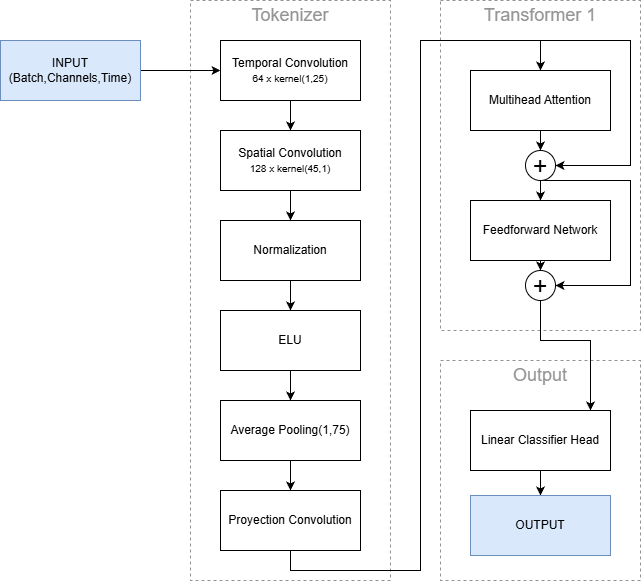
\includegraphics[width=\textwidth]{Imagenes/Bitmap/Esquema-Modelo}
	\caption{Esquema de la arquitectura de MiRepNet para clasificación.}
	\label{fig:esquemaModelo}
\end{figure}

Tras la fase de pretraining, se deja de aplicar el enmascaramiento de tokens y se elimina el segundo bloque Transformer encargado de la reconstrucción, manteniéndose únicamente el Transformer principal junto con la capa lineal de clasificación. Este Transformer ha aprendido representaciones generales de las señales EEG, que pueden ser reutilizadas en tareas específicas.

Para adaptar el modelo a un sujeto concreto, es necesario realizar una fase de fine-tuning, en la que el modelo se entrena utilizando datos del propio usuario. Durante esta fase, es posible optar por congelar los pesos del Transformer, manteniendo así las representaciones generales aprendidas durante el preentrenamiento, o bien permitir su actualización.

En los experimentos realizados, se ha observado que congelar el Transformer conlleva una disminución significativa del rendimiento. Esto sugiere que, a pesar de haber aprendido patrones generales, resulta necesario ajustar el modelo a las características específicas de cada sujeto.

\subsection{Implementación}
\label{subsec:implementacionModelo}

Tanto la arquitectura del modelo como sus pesos iniciales fueron obtenidos a partir del repositorio oficial de MiRepNet. Con el objetivo de facilitar la extensibilidad del sistema y permitir la sustitución del modelo por alternativas en el futuro, se diseñó una interfaz denominada ModelInterface, encargada de encapsular la funcionalidad principal del modelo.

Esta interfaz define un conjunto de métodos comunes, entre los que se incluyen: \texttt{predict}, \texttt{predict\_batch}, \texttt{finetune}, \texttt{save} y \texttt{get\_constructor\_params}. De este modo, se establece una capa de abstracción que desacopla el uso del modelo de su implementación concreta.

La implementación de estos métodos se llevó a cabo en ausencia de documentación detallada, basándose en el análisis del código disponible en el repositorio oficial de MiRepNet.
